\chapter{Related Work}
\label{ch:related_work}

\section{Path Following Methods}
\label{sec:path_following_methods}

There are different methods in the field of path-following control. Such as Vector field, Virtual target pursuit, Nonlinear, Feedback linearization, Optimal control, Model predictive control to name a few.

\subsection{Vector Field Method}
\label{subsec:vector_field_method}

\begin{figure}[h] % Fix position in document via 'h'
    \centering
    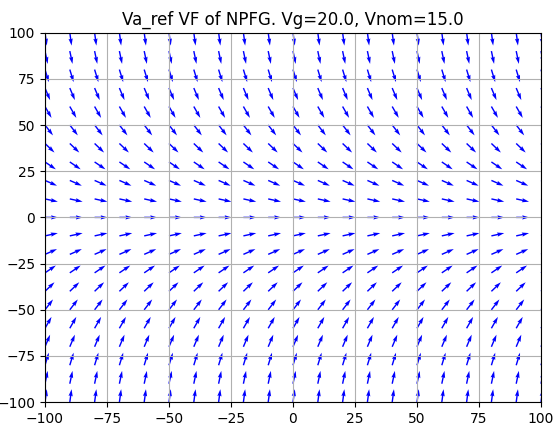
\includegraphics[width=0.7\textwidth]{vector_field_method_example}
    \caption{Visual representation of a Vector Field. Path is at Y=0 with the direction of +X}
\label{fig:vf_example}
\end{figure}

Vector Field method is based on generating a field of vectors around the path that when the vehicle follows the directions defined by the vectors, it will converge to the path\cite{stastny_flying_2019}\cite{sharma_vector_nodate}.\\

Since the Vector Field approach is simple (geometry), and easily extendable (vector field can be interpreted by both multirotor and fixed wing), it was chosen as the basis for the formulation in this thesis.

\subsection{Virtual Target Pursuit Method}
One of the most intuitive way to achieve path following is to have a virtual target point on the path that the vehicle chases. Also known as 'carrot chasing' method (imagine placing a carrot, and a horse blindly follows it. If you can steer the carrot cleverly, you can have an accurately path-following horse!), this method includes for example widely used L1 guidance law\cite{park_new_2004}, especially for fixed wing and multirotor applications in open-source autopilot software.

\section{Path Following on Hybrid VTOL}
Although almost no research on using a unified path following guidance for a Hybrid VTOL was conducted in the past, one study\cite{zhou_incremental_nodate} showed an 'Incremental nonlinear dynamic inversion' based path following for both multirotor and fixed-wing modes operation of a hybrid quad-plane. This study utilized the same concept as this thesis of the Vector Field method to generate desired ground velocity vector.\\

However, it assumed an arbitrary constant speed of 2.0 m/s for a multirotor, which severely under-utilizes the wide speed range of a multirotor. Also, having a constant speed means the ground track of converging to the path will always form arcs, which is also not how an operator would assume the vehicle to move and is severely under-utilizing the omnidirectional acceleration capability of a multirotor.